\chapter{TECNOLOGIAS E FERRAMENTAS UTILIZADAS}
\label{cap:TECNOLOGIAS-E-FERRAMENTAS-UTILIZADAS}


\section{Unity 3D – Ambiente de Desenvolvimento}
\label{sec:Unity-3D-–-Ambiente-de-Desenvolvimento}

Unity é uma ferramenta com múltiplas utilidades na qual permite o usuário a desenvolver desde um jogo simples até de um de última geração.
Segundo o próprio site onde é fornecida a ferramenta "O Unity é um motor de desenvolvimento integrado que fornece uma funcionalidade pioneira para criação de jogos e outros conteúdos interativos. Poderá utilizar o Unity para montar sua arte e recursos em cenas e ambientes; adicionar física, editar e testar simultaneamente seu jogo e, quando preparado, publicar em suas plataformas escolhidas, tais como computadores fixos, a rede, iOS, Android, Wii, PS3 e Xbox 360." (Unity3D).
O Unity suporta três linguagens de programação que são Boo, JavaScript e o C#, esta última sendo utilizada para desenvolvimento do jogo Caapora. O Unity também possui módulos que podem ser instalados possibilitando o desenvolvimento sem linha de código.


	\begin{figure}[h!]
		\centering
		\Caption{\label{fig:exemplo-1} Lorem ipsum dolor sit amet, consectetur adipiscing elit. Suspendisse commodo lectus et augue elementum varius.}	
		\UECEfig{}{
			\fbox{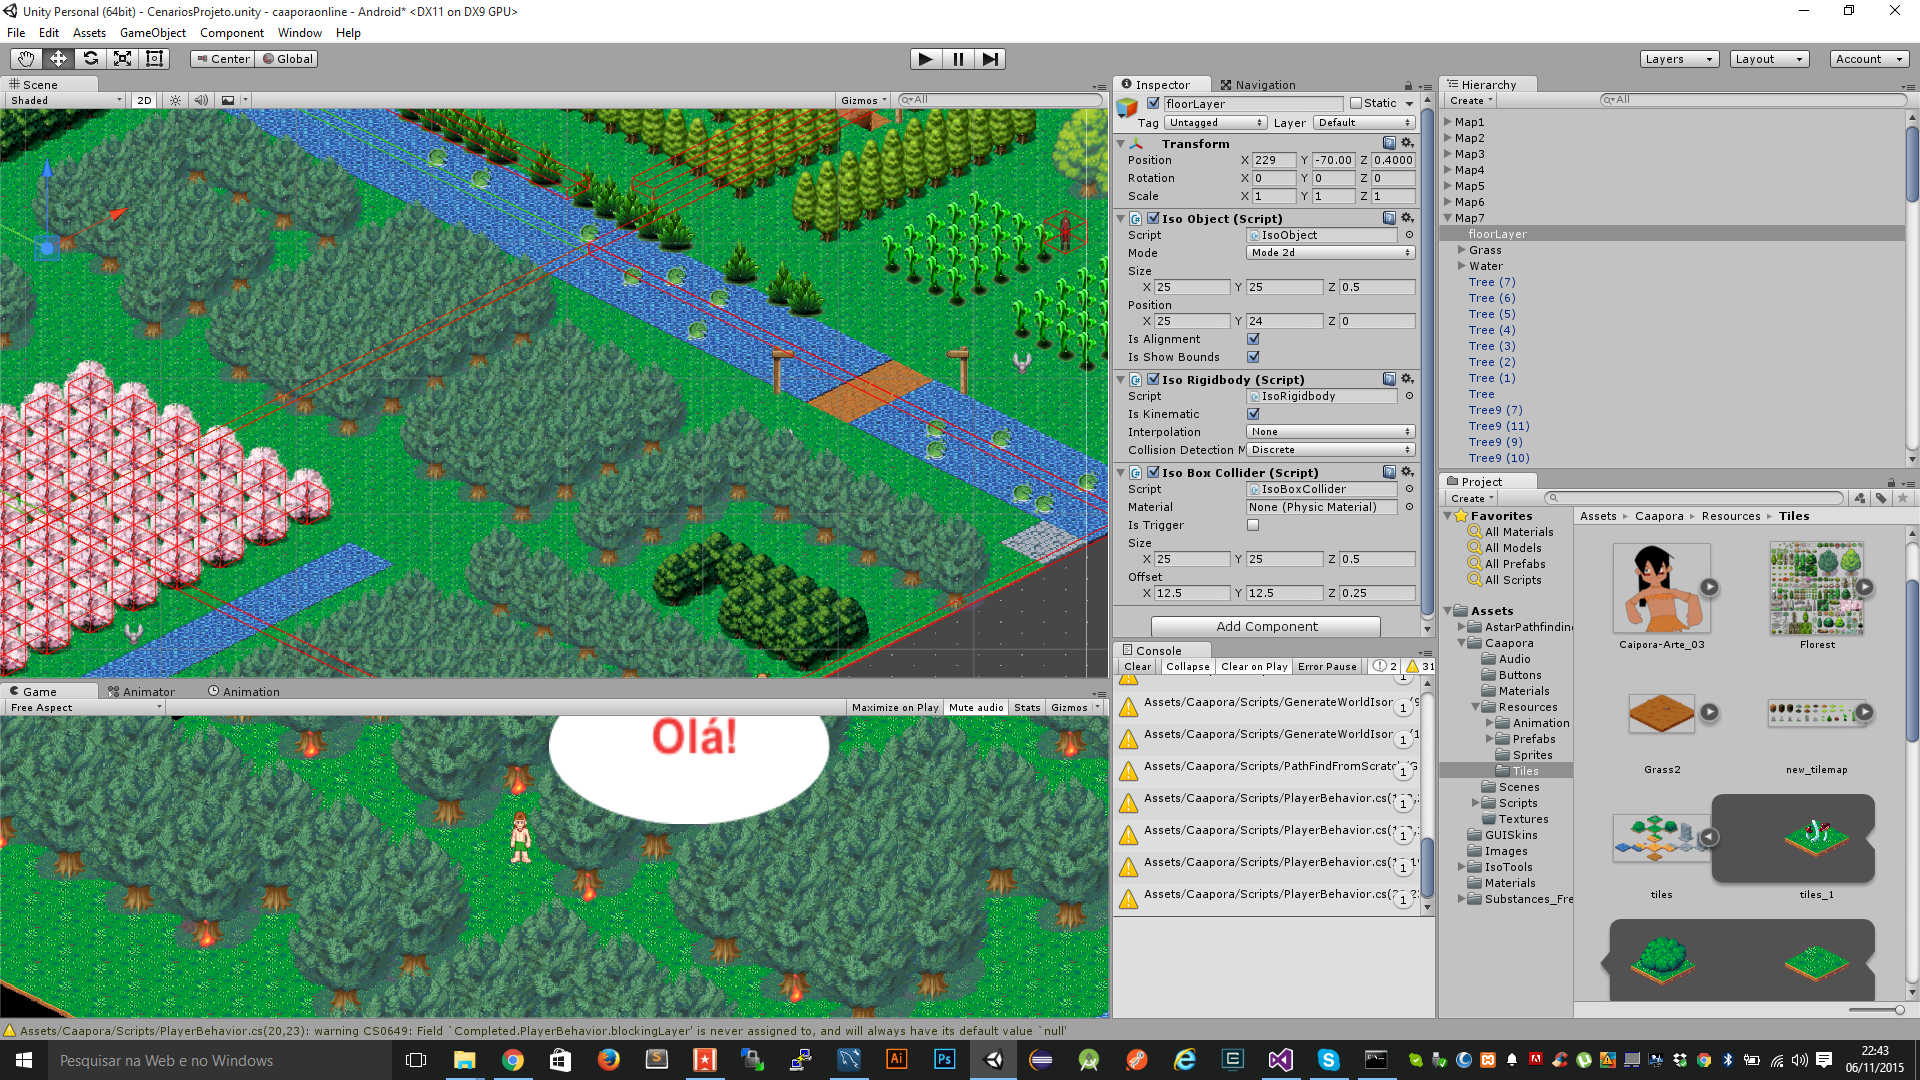
\includegraphics[width=10cm]{figuras/Unity}}
		}{
			\Fonte{Elaborado pelo autor}
		}	
	\end{figure}
	
Umas das principais vantagens de se utilizar o Unity é a possibilidade de desenvolver o jogo uma única vez e poder utiliza-lo em mais de 10 plataformas diferentes sem as necessidades de alterar o produto inicial. 
Algumas destas plataformas são: iPads, PC e iPhone

	
\section{Linguagem de programação Java Script}
\label{sec:Linguagem-de-programação-Java-Script}

JavaScript é uma linguagem para auxilio na criação de Home-Pages, as funções escritas em JavaScript podem ser embutidas dentro de seu documento HTML, possibilitando o incremento das funcionalidades do seu documento HTML com elementos interessantes. Sendo possivel: responder facilmente a eventos iniciados pelo usuário, incluir efeitos que tornem sua página dinâmica. Logo, podemos criar sofisticadas páginas com a ajuda desta linguagem. (GONÇALVES, 2005)

JavaScript é uma linguagem de programação criada por Brendan Eich em 1995, é uma linguagem dinâmica, orientada a objetos e possui similaridades com a linguagem C. 
É uma linguagem baseada em scripts e tem como sua principal característica em ser executado localmente, no lado do cliente, excluindo a necessidade de um servidor remoto.
Podemos dizer que JavaScript é mais uma extensão do HTML do que uma linguagem de programação propriamente dita. O primeiro browser a suportar JavaScript foi o Netscape Navigator 2.0 (GONÇALVES, 2005)

\section{Linguagem de programação Csharp}
\label{sec:Linguagem-de-programação-Csharp}

C# é uma linguagem elegante e de tipos protegidos, orientada a objeto e que permite aos desenvolvedores construírem uma variedade de aplicações seguras e robustas, compatíveis com o .NET Framework. É possível usar C# para criar muito aplicativos de cliente do Windows, serviços Web XML, componentes distribuídos, aplicativos de cliente-servidor, aplicativos de banco de dados, e muito mais. O Visual Csharp fornece um editor de códigos avançado, designers de interface de usuário convenientes, depurador integrado, e muitas outras ferramentas para facilitar o desenvolvimento de aplicativos baseados na linguagem C# e no .NET Framework. (MICROSOFT, 2015)

A linguagem Csharp foi desenvolvida pela Microsoft para ser um farmework .NET. 
O Csharp é similar ao C++ e Java, sendo também uma linguagem fortemente tipada, orientada a objeto, portanto suporta heranças, polimorfismo e encapsulamento. 
Algumas características desta linguagem: 

\begin{alineascomponto}
	\item Controle de versão: cada assembly gerado, seja como EXE ou DLL, tem informação sobre a versão do código. 

	\item Orientada a objetos: em C#, qualquer variável tem de fazer parte de uma classe.  

	\item Linguagem gerenciada: todo gerenciamento de memória é feito pelo runtimevia GC (GarbageColletor), e não diretamente pelo programador, reduzindo assim as chances de cometer erros comuns.


Nunc ac pretium dui. Mauris aliquam dapibus nulla ac mattis. Aenean non tortor volutpat, varius lectus vitae, accumsan nibh. Cras pretium vestibulum enim, id ullamcorper tortor ultrices non. Integer sodales viverra faucibus. Curabitur at dui lacinia, rhoncus lacus at, blandit metus. Integer scelerisque non enim quis ornare.

	\begin{quadro}[h!]	
		\centering
		\Caption{\label{qua:exemplo-1} Praesent ex velit, pulvinar at massa vel, fermentum dictum mauris. Ut feugiat accumsan augue}		
		\UECEqua{}{
			\begin{tabular}{|c|c|l|l|}
				\hline
				Quisque & pharetra & tempus & vulputate \\
				\hline
				E1 & Complete coverage by a single transcript & Both  & Complete\\
				\hline
				E2 & Complete coverage by more than & Both splice sites & Complete\\
				\hline
				E3 & Partial coverage & Both splice sites & Both \\				
				\hline
			\end{tabular}
		}{
			\Fonte{Elaborado pelo autor}
		}
	\end{quadro}
	
\lipsum[20]

	
	\begin{quadro}[h!]	
		\centering
		\Caption{\label{qua:exemplo-2} Duis faucibus, enim quis tincidunt pellentesque}		
		\UECEqua{}{
			\begin{tabular}{|c|c|}
				\hline
				Quisque & pharetra \\
				\hline
				E1 & Complete coverage by a single transcript \\
				\hline
				E2 & Complete coverage by more than \\
				\hline
				E3 & Partial coverage \\
				\hline
				E4 & Partial coverage \\
				\hline
				E5 & Partial coverage \\
				\hline
				E6 & Partial coverage \\
				\hline
				E7 & Partial coverage \\
				\hline
			\end{tabular}
		}{
			\Fonte{Elaborado pelo autor}
		}
	\end{quadro}

\lipsum[21]

Integer non lacinia magna. Aenean tempor lorem tellus, non sodales nisl commodo ut. Proin mattis placerat risus sit amet laoreet. Praesent sapien arcu, maximus ac fringilla efficitur, vulputate faucibus sem. Donec aliquet velit eros, sit amet elementum dolor pharetra eget. Integer eget mattis libero.
\Gls{ambiguidade}
\Gls{braile}
\Gls{coerencia}
\Gls{dialetos}
\Gls{elipse}
\Gls{locucao-adjetiva}
\Gls{modificadores}
\Gls{paronimos}
\Gls{sintese}
\Gls{borboleta}